A key step for obtaining computational proofs of geometric results is a discretization of the space or the problem at hand. For example, a priori it could be that the only set of points in $\mathbb{R}^2$ that holds a particular property requires all points to have non-computable coordinates. Fortunately, this is not the case for Erd\H{o}s-Szekeres-type problems, where the properties of interest (e.g., convexity, emptiness) are invariant under rotations, translations, and even small perturbations of the coordinates. 
The combinatorial abstraction that has been most widely used in this context is that of \emph{triple orientations}~\cite{ emptyHexagonNumber, scheucherTwoDisjoint5holes2020}, also known as \emph{signotopes}~\cite{felsnerSweepsArrangementsSignotopes2001, subercaseaux2023minimizing},  Knuth's \emph{counterclockwise} relation~\cite{knuthAxiomsHulls1992}, or \emph{signatures}~\cite{szekeres_peters_2006}. Given points $p, q, r$, their \emph{triple-orientation} is defined as 
\newcommand{\sign}{\operatorname{sign}}
\[
  \sigma(p, q, r) = \sign \det \begin{pmatrix} p_x & q_x & r_x \\ p_y & q_y & r_y \\ 1 & 1 & 1 \end{pmatrix} = \begin{cases}
    1 & \text{if } p, q, r \text{ are \emph{oriented} counterclockwise}, \\
    0 & \text{if } p, q, r \text{ are collinear}, \\
    -1 & \text{if } p, q, r \text{ are \emph{oriented} clockwise}.
  \end{cases}.
\]

\begin{figure}
  \centering
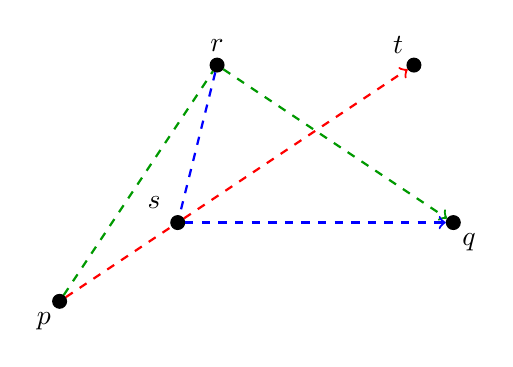
\begin{tikzpicture}
  %\draw[ultra thick, dashed, blue] (5,1) -- (0,0);
  \node[draw, circle, black, fill=black, inner sep=0pt, minimum size=5pt] (p) at (0,0) {};
  \node[] at (-0.2, -0.25) {$p$};
  \node[draw, circle, black, fill=black, inner sep=0pt, minimum size=5pt] (q) at (5,1) {};
  \node[] at (5.2, 0.75) {$q$};
  \node[draw, circle, black, fill=black, inner sep=0pt, minimum size=5pt] (r) at (2,3) {};
  \node[] at (2, 3.25) {$r$};

  \node[draw, circle, black, fill=black, inner sep=0pt, minimum size=5pt] (s) at (1.5, 1) {};
  \node[] at (1.2, 1.25) {$s$};

  \node[draw, circle, black, fill=black, inner sep=0pt, minimum size=5pt] (t) at (4.5, 3) {};
  \node[] at (4.3, 3.25) {$t$};

  \draw[ thick, dashed, green!60!black] (p) -- (r);
  \draw[ thick, dashed, green!60!black, ->] (r) -- (q);

  \draw[ thick, dashed, blue] (r) -- (s);
  \draw[ thick, dashed, blue, ->] (s) -- (q);

  \draw[thick, dashed, red] (p) -- (s);
  \draw[thick, dashed, red, ->] (s) -- (t);
  % \draw[fill=green, opacity=0.5] (a.center) -- (b.center) -- (c.center) -- cycle;
\end{tikzpicture}
\caption{Illustration of triple orientations, where $\sigma(p, r, q) = -1, \sigma(r, s, q) = 1, $ and $\sigma(p, s, t) = 0$.}\label{fig:triple-orientation} 
\end{figure}

An example is illustrated in~\Cref{fig:triple-orientation}. Formally, we identify points with members of $\mathbb{R}^2$, and use \textsf{mathlib}'s definition of the determinant to define $\sigma$.
\begin{lstlisting}
abbrev Point := EuclideanSpace ℝ (Fin 2)
@[pp_dot] abbrev x (p : Point) : ℝ := p 0
@[pp_dot] abbrev y (p : Point) : ℝ := p 1

inductive Orientation : Type
  | CW -- clockwise :=  -
  | CCW -- counter clockwise:= +
  | Collinear -- := 0
  deriving DecidableEq

def Orientation.ofReal (r : ℝ) : Orientation :=
  if 0 < r then CCW
  else if r < 0 then CW
  else Collinear

noncomputable def σ (p q r : Point) : Orientation :=
  .ofReal Matrix.det !![p.x, q.x, r.x ; p.y, q.y, r.y ; 1, 1, 1]
\end{lstlisting}

With the $\sigma$ function we can immediately define the notion of \emph{general position} for collections (e.g., finite sets, lists, etc.) of points, simply establishing that $\sigma(p, q, r) \neq 0$ for every triple of points $p, q, r$ in the collection.
We can now start formalizing sets of points that are \emph{equivalent} with respect to their triple orientations, and consequently, properties of pointsets that are fully captured by their triple orientations~(\emph{orientation properties}).

\begin{lstlisting}
  structure σEquiv (S T : List Point) :=
    (f : Point → Point)
    (perm : S.map f ~ T)
    (σ : ∀ p q r, p ∈ S → q ∈ S → r ∈ S → σ (f p) (f q) (f r) = σ p q r)

  def OrientationProperty (P : List Point → Prop) :=
    ∀ {{S T}}, S ~σ T → (P S ↔ P T) -- `~σ` is infix notation for `σEquiv`
\end{lstlisting}

